\chapter{Industrial PID Control}
\label{chap:IndustrialPID}
\abstract*{abstract (10--15 lines long)}

\abstract{abstract (10--15 lines long)}

\section{Control System Design Scenario}
\label{sec:1}

Control systems are used to maintain process conditions at their desired values by manipulating certain process variables to adjust the variables of interest. A common example of a control system from everyday life is the cruise control on an automobile. The purpose of a cruise control is to maintain the speed of the vehicle (the controlled variable) at the desired value (the set point) despite variations in terrain, hills, etc. (disturbances) by adjusting the throttle, or the fuel flow to the engine (the manipulated variable). Another example is the home thermostat. This control system is designed to maintain the temperature in the home at a comfortable value by manipulating the fuel flow or electrical input to the furnace. The furnace control system must deal with a variety of disturbances to maintain temperature in the house, such as heat losses, doors being opened and hope- fully closed, and leaky inefficient windows. The furnace must also be able to respond to a request to raise the desired temperature if necessary. For example, we might desire to raise the temperature by 5 degrees and we would like the system to respond smoothly and efficiently. From these examples, we can deduce that there are several common attributes of control systems:
\begin{itemize}
\item The ability to maintain the process variable at its desired value in spite of disturbances that might be experienced (this is termed disturbance rejection)
\item The ability to move the process variable from one setting to a new desired setting (this is termed set point tracking)
\end{itemize}

\begin{figure}[tb]
\centering
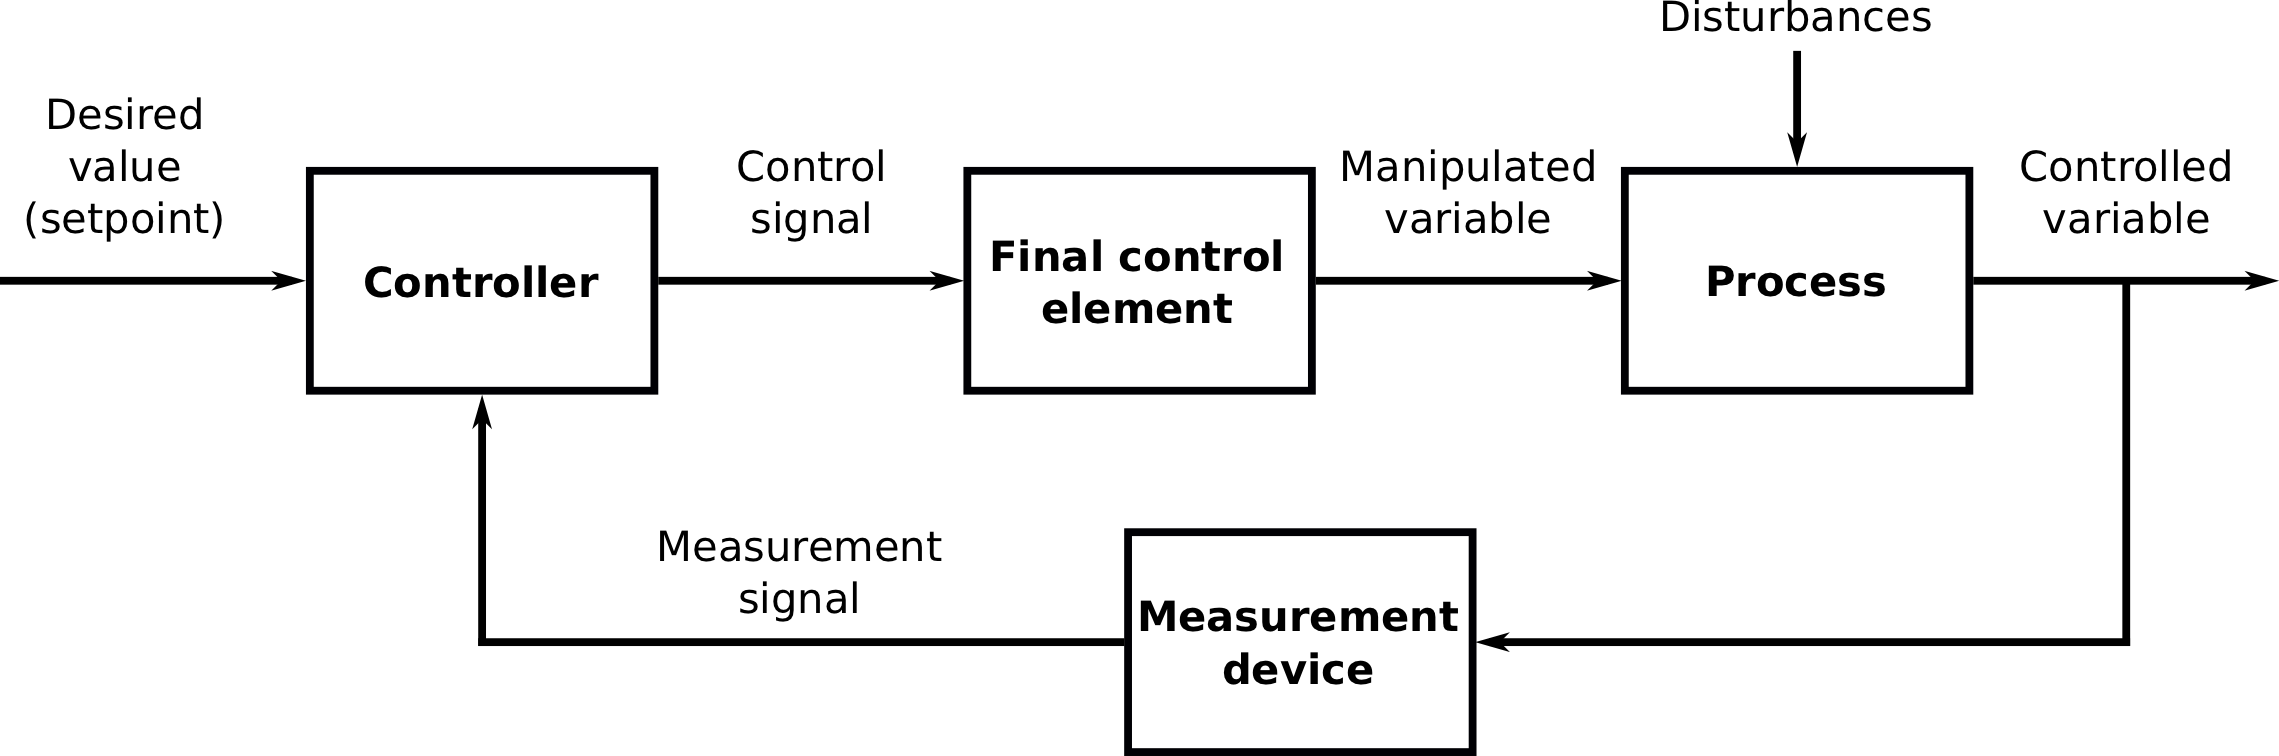
\includegraphics[width=0.8\linewidth]{Ch2FeedbackControlSystem}
\caption{Feedback Control System} \label{Ch2fig:FeedbackControlSystem}
\end{figure}

\begin{figure}[tb]
\centering
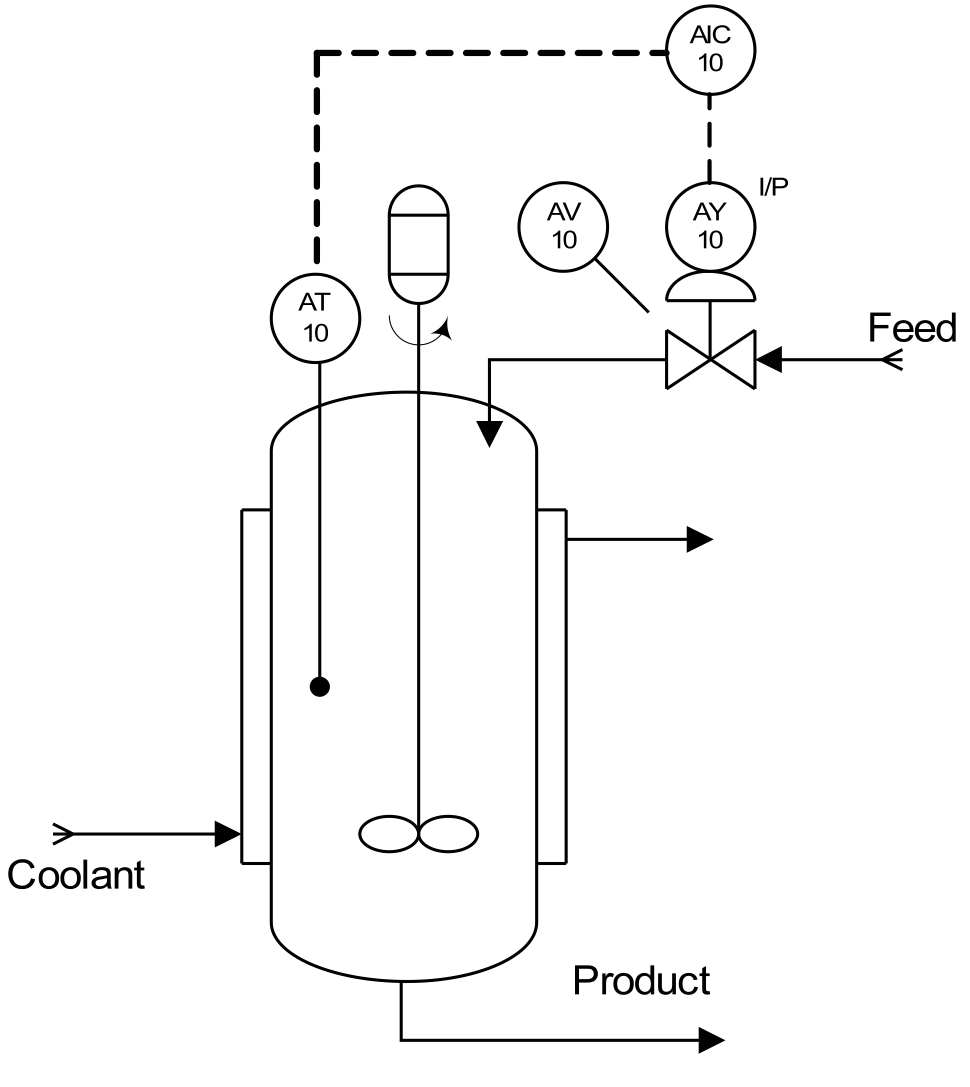
\includegraphics[width=0.4\linewidth]{Ch2Reactor}
\caption{Isothermal Continuous Stirred Tank Reactor (CSTR)} 
\label{Ch2fig:CSTR}
\end{figure}

A natural way to adjust or correct the behaviour over time of a dynamic system output, the controlled variable, is by using an actuating input computed on the basis of the comparison of the actual output with its desired value: the feedback error. This is, by means of closed-loop control. To compute the control action information about the feedback error evolution is required. Normally its current value, its past evolution, and a prediction of its future behaviour are used. The way we use this information to deliver the control action constitutes the control algorithm. Conceptually we can view the control systems in the general manner shown in figure (\ref{Ch2fig:FeedbackControlSystem}). As a detailed  practical example, consider the isothermal Continuous Stirred Tank Reactor (CSTR), as the one in figure (\ref{Ch2fig:CSTR}), where the isothermal series/ parallel Van de Vusse reaction takes place \cite{arrietaETFA2008}, \cite{VandeVusse2} . The reaction can be described by the following scheme

\begin{align}
    A \overset{k_1}{\longrightarrow} B \overset{k_2}{\longrightarrow}C\\
    2 A \overset{k_3}{\longrightarrow} D \nonumber
\end{align}


From a mass balance, the system can be described by the following model

\begin{align}
    \frac{dC_A(t)}{dt} & = \frac{F_r(t)}{V} \left[C_{Ai}-C_A(t)\right] - k_1 C_A(t) - k_3 C^2_A(t) \nonumber \\
    \frac{dC_B(t)}{dt} & = -\frac{F_r(t)}{V} C_B(t)+ k_1 C_A(t) - k_2 C_B(t)
    \label{Ch2eq:system3}
\end{align}

\noindent where $F_r$ is the feed flow rate of product $A$, $V$ is the reactor volume which is kept constant during the operation, $C_A$ and $C_B$ are the reactant concentrations in the reactor, and $k_i$ ($i=1,2,3$) are the reaction rate constants for the three reactions.\\



From the point of view of the feedback control system depicted in figure (\ref{Ch2fig:FeedbackControlSystem}), the controlled variable is the product concentration $C_B$, the manipulated variable  the feed flow rate $F_r$. Expected disturbances on the system  may come from variations on the input product concentration $C_A$ as well as flow rate. In figure (\ref{Ch2fig:CSTRFigureOpenLoop}) we can observe how the reactor output concentration reacts to changes in each one of its two inputs: The inlet flow rate, $F_r$ and concentration $C_A$. Whereas the first one can be manipulated the second one is considered now know as supplied externally. Therefore, $F_r$ is considered as the manipulated variable and will be the one used to operate and control the reactor. On the other hand, changes in $C_A$ will be seen as disturbances and the controller should be able to counteract such changes and prevent them to generate changes in the output concentration $C_B$. 

\begin{figure}[htb]
\centering
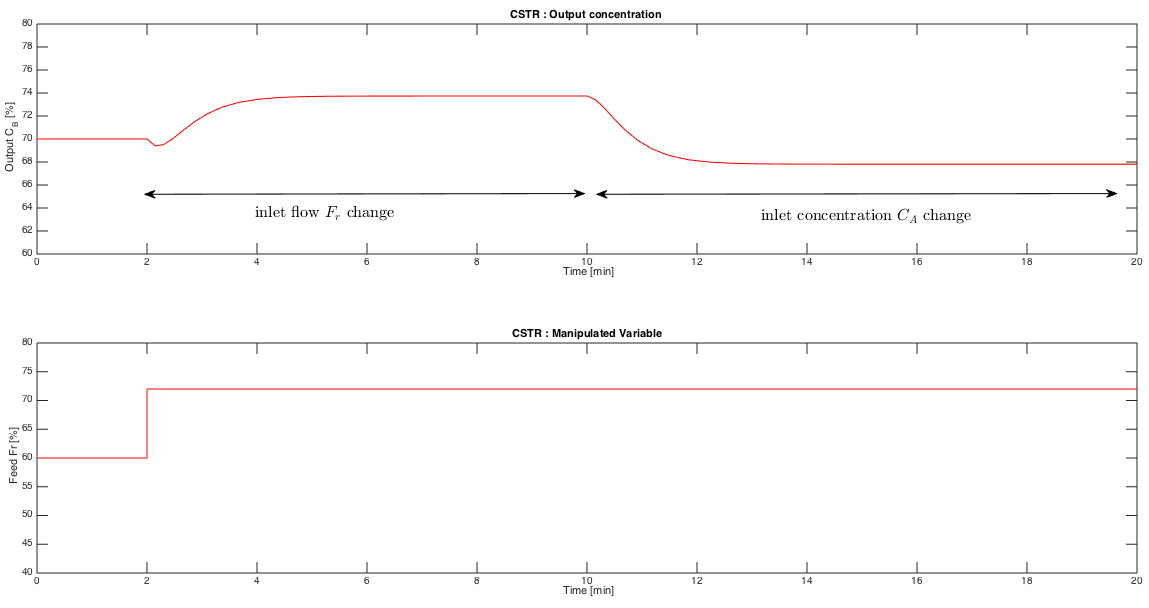
\includegraphics[width=0.9\linewidth]{../figuras/Ch2FigureOpenLoop}
\caption{CSTR Open-loop output to change sin inlet flow and concentration} 
\label{Ch2fig:CSTRFigureOpenLoop}
\end{figure}


The feedback control structure has been used for a long time, but if we constraint ourselves to the industrial process control area, the proportional (present) integral (past) derivative (future) (PID) control algorithm age starts in the 40's  with the PID controller and this will be the concern of this text.  A control algorithm has a number of control parameters, which must be \emph{tuned} (adjusted) to have acceptable performance. Often the tuning is done on a simulation model before implementing the control strategy on the actual process. In this text ww will concentrate on the determination of the controller tuning, in fact, PID tuning, by means of optimisation methods. Specifically, optimisation methods that deal with multiple objectives at the same time. However, prior to this task, we should define the control scenario where the design will take place.\\

Consider the general two-degree-of-freedom closed-loop control system depicted in figure~\ref{Ch2fig:DoFControlSystem} where $P(s)$ and $\{C_r(s), C_y(s)\}$ are the controlled process model and the controller transfer functions, respectively.  In this system, $r(s)$ is the set-point, $u(s)$ the controller output signal, $d(s)$ the disturbance, $y(s)$ the process controlled variable, and $n(s)$ the measurement noise. It is assumed that the disturbance enter at the process input (load-disturbance).

\begin{figure}[htb]
\centering
	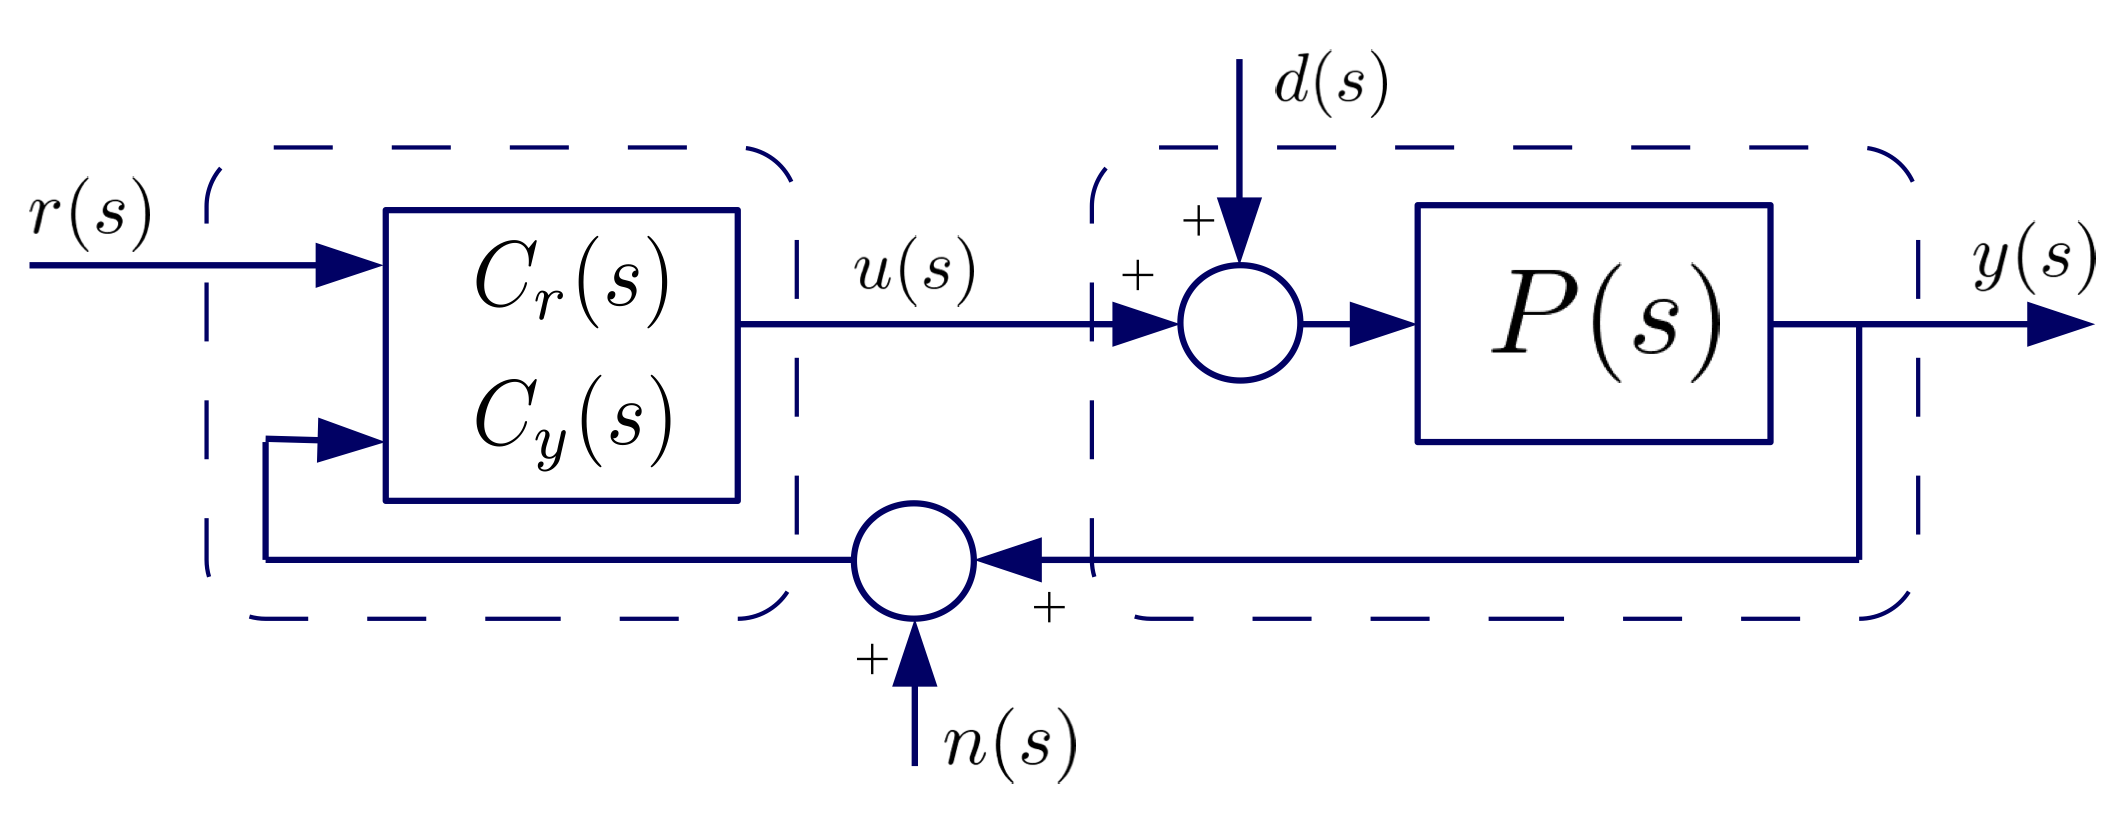
\includegraphics[width=0.8\linewidth]{../figuras/Ch2DoFControlSystem} 
\caption{Two-Degree-of-freedom closed-loop control system.} 
\label{Ch2fig:DoFControlSystem}
\end{figure}


The closed-loop control system output $y(s)$ as a function of its inputs $r(s)$, $d(s)$, and $n(s)$ is

\begin{equation}
	y(s) = M_{yr}(s) r(s) + M_{yd}(s) d(s) + M_{yn}(s) n(s), \label{Ch2eq:yt}
\end{equation}

\noindent where
\begin{equation}
	M_{yr}(s) \doteq \frac{C_r(s)P(s)}{1+C_y(s)P(s)}, \label{Ch2eq:myr}
\end{equation}

\noindent is the servo-control closed-loop transfer function, 
\begin{equation}
	M_{yd}(s) \doteq \frac{P(s)}{1+C_y(s)P(s)}, \label{Ch2eq:myd}
\end{equation}

\noindent the regulatory control closed-loop transfer function, and
\begin{equation}
	M_{yn}(s) \doteq \frac{-C_y(s)P(s)}{1+C_y(s)P(s)}, \label{Ch2eq:myn}
\end{equation}

\noindent the measurement noise sensitivity function.\\

The regulatory control main objective is \emph{load-disturbance rejection}; this is, to return the controlled variable to its set-point in the event a disturbance enters to the control system.  For the servo-control, it is intended to \emph{follow a changing set-point}; this its, to bring the controlled variable to its new desired value. Controller tuning for above operations must take also into account to not amplified the measurement noise, if any.  In figure (\ref{Ch2fig:CSTRFigureClosedLoop}) we can see the CSRT example presented above, where a controller, is accomplishing the task of, first, tracking a set-point step change of, followed by a disturbance attenuation  of two changes. One  in the concentration, $C_{Ai}$, of $A$ in the feed flow and finally a change in the supplied flow rate.

\begin{figure}[tb]
\centering
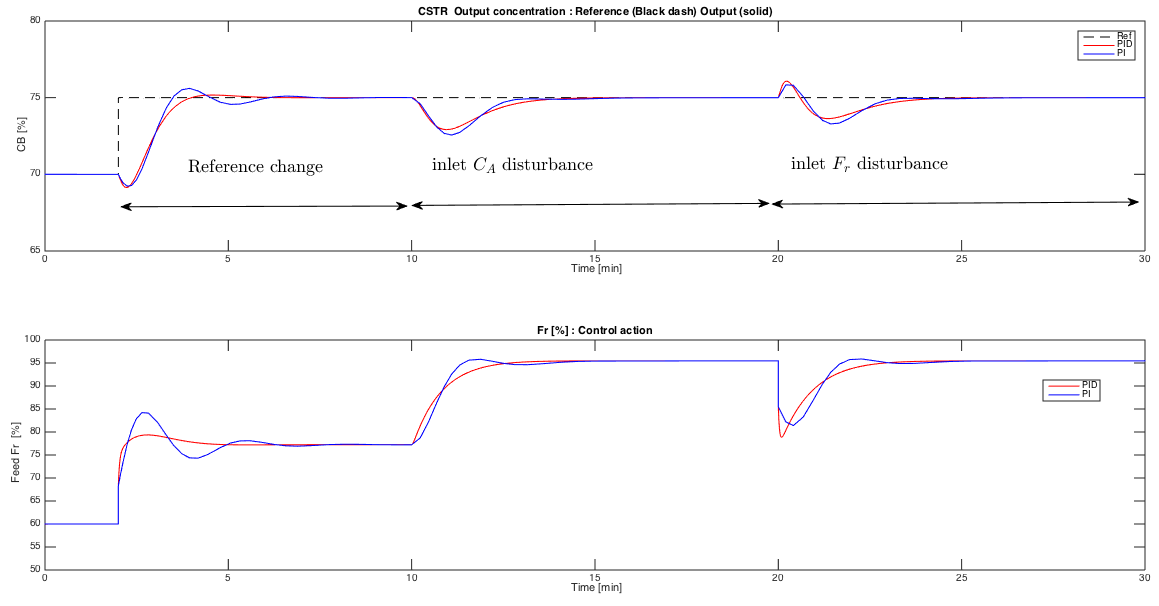
\includegraphics[width=0.9\linewidth]{../figuras/Ch2FigureClosedLoop}
\caption{CSTR Open-loop output to disturbance changes in inlet flow and concentration} 
\label{Ch2fig:CSTRFigureClosedLoop}
\end{figure}


\section{Industrial Process Characteristics}
\label{sec:2}

Before a controller for a process is specified, the process to be controlled should be characterised, at least in some broad sense. There are many different types of processes that are controlled automatically. Examples range from fluid levels in tanks to read-write heads of computer disk storage devices. The control inputs to a process are supplied through one or more actuators. For example a motor driven valve can be an actuator for fluid flowing into a tank. Process outputs that are being controlled (e.g., the fluid level in a tank) are measured using appropriate sensors. The basic control of one output variable by the use of one control input variable is called single-input single-output (SISO) control. For more complex systems, multi-input multi-output (MIMO) control may be required. PID control was developed initially as a SISO control strategy, but it has been extended in various ways to MIMO control \cite{wang2008}. Event these extensions, it is common practice in the process industry to rely on PID control at single loop level control problems, whereas multivariable control solutions, such as model predictive control are the ones applied for multivariable and supervisory control \cite{VilanovaBook2012}.\\

In the great majority of process loops, applying a step to the control variable causes the controlled variable to reach a steady state and does not provoke an instantaneous variation of it. This means that the process model seen by the regulator can be described by an asymptotically stable, strictly proper transfer function. FOPTD dynamics are probably the most usual models used in the process industry for modelling self-regulating behaviours. For example when modelling dynamics that involve balances of temperature, matter, and energy in general. Also in a reactor where a reaction takes place, the components balance generates a dynamics that can be usually modelled as a FOPTD. When different reactors are connected in series, higher order systems arise that can be described by SOPTD models. \\

In a few loops, a control step causes the controlled variable to asymptotically assume a ramp-like behaviour. This case is commonly referred to as  integrating or non self-regulating processes. These dynamics arises, for example, when dealing with level problems. Also when dealing with distillation columns control problems, integrative behaviour arises. Other cases (e.g. an oscillatory response with significant delay, unstable dynamics, etc) may exist, but they are unlikely to appear in practice. This is what motivates the current approaches to PID control to concentrate on stable self-regulating dynamics and these are the process models adopted in this book to define the working scenario. However, from the provided methodology and tools it should become clear that the work could be extended to some other process dynamics.  \\

A complete and illustrative source of modelling for process control, illustrating how the previously commented dynamics arise is the extensive book \cite{MarlinBook}, , whereas industrial applications can be sourced, for example, in  \cite{VilanovaBook2012}.


\subsection{Controlled Process Model}
\label{sec:2.1}

The simple structure of the PID controller calls for simple process descriptions, this fact motivates the use of first or second order models. On that respect, the controlled process model in the control design scenario considered in this book will be the one aimed at representing the self-regulating non-oscilating (overdamped) step responses. The overdamped controlled processes will be represented by a linear model given by the transfer function

\begin{equation}
    P(s) = \frac{K_p e^{-Ls}}{(Ts+1)(aTs+1)}, \ \tau_o = L/T 
    \label{Ch2eq:SOPTD}
\end{equation}

\noindent where $K_p$ is the model gain, $T$ its main time constant, $a$ the ratio of its two time constants ($0 \leq a \leq 1.0$), $L$ its dead-time, and $\tau_o$ the model \emph{normalized dead-time} ($0.1 \leq \tau_o \leq 2.0$). Model transfer function \eqref{Ch2eq:SOPTD} allows to represent First-Order-Plus-Dead-Time (FOPDT) processes, with $a=0$, over damped Second-Order-Plus-Dead-Time (SOPDT) processes, with $0 < a < 1$, and Dual-Pole-Plus-Dead-Time (DPPDT) processes, the $a=1$ case.\\

In the great majority of cases, a process description is obtained by performing an experiment on the process. In most cases, a step response will be used. They are also easy to apply. It suffices to switch the regulator to manual, wait until a reasonably steady state is reached, then change the control variable suddenly by an amount sufficient to make the response obtained easily distinguishable from noise. In addition, step tests permit the process to be maintained under reasonable control without perturbing it excessively or leading it to the stability boundary, as required e.g. by the closed loop Ziegler-Nichols method \cite{astromhagglund2006}. From this point of view, to maintain the need for plant experimentation to a minimum is a key point when considering the industrial application of a technique. The parameters of the controlled process model \eqref{Ch2eq:SOPTD}, $\overline{\theta}_p = \left\{K_p, T, a, L, \tau_o \right\}$, may be identified from the process reaction curve by using, for example, the method presented in \cite{alfaro2006-1}. 



\section{The PID Controller}
\label{sec:3}
Undoubtedly, since its introduction, PID controllers are the option most frequently used in different process control applications. Their success is mainly due to the simplicity of their structure (three parameters to tune) and operation, which allows the control engineer a better understanding compared with other advanced control techniques. This has motivated the continuous research efforts aimed at finding alternative approaches to the design and new tun- ing rules in order to improve the performance of control loops based on PID controllers. Different reports confirm that currently the PID continues to be the workhorse of process industry, being completely integrated within more advanced control algorithms and providing the fundamental base layer for plant-wide solutions. The proper function of a PID- based control loop is, therefore, a key aspect in the current process industry and of continuing interest for researchers.\\

The application of a PID controller is, essentially, the result of weighting three different actions each one of them related to the information provided by the time history of the error signal: the instantaneous actual value provided by the  \emph{proportional term}, $u_P(t)$, past values provided by the \emph{integral term}, $u_I(t)$, and the predicted future values provided by the \emph{derivative term}, $u_D(t)$.  In its simplest form, the PID control signal is computed as

\begin{equation}
u(t)=u_P(t)+u_I(t)+u_D(t)= K_p \left ( e(t)+\frac{1}{T_i}\int_0^t e(\tau)\md \tau+T_d\frac{\md}{\md t}e(t) \right )
\end{equation}

\noindent which corresponds, when expressed in the form of the transfer function from the error $e(s)$ to $u(s)$, to

\begin{equation}
u(s)=K_p \left ( 1+\frac{1}{T_is}+{T_ds} \right )  e(s)
\label{Ch2eq:PID_ideal}
\end{equation}

This form is usually referred to as the \emph{ideal} PID. The three-term functionalities are highlighted by the following.

\subsubsection*{Proportional term}

Also referred as the P mode, this mode is almost universal and present in all controllers. With reference to \eqref{Ch2eq:PID_ideal}, the control law in this case is given by

\[u_P (t) = K_pe(t) + u_{ss}\]

\noindent where $u_P(t)$ is the (proportional) controller output, $K_p$ is the controller gain and $u_{ss}$ is a bias or reset value. The P action makes the control proportional to the error. Hence it obeys to the intuitive principle that, the bigger the error the bigger the control action must be.\\

The P action depends only on the instantaneous value of the error and is nonzero only if $e(t)$ is nonzero. In other words, the P action is ideally zero at steady state, but only provided that the required steady state can be reached with zero control. If this is not the case it will be necessary to \emph{reset} $u(t)$, i.e. to add a constant term to it so that it maintains the required steady state; if only the P action is used, this is the role of $u_{ss}$. However, the reset can also be accomplished by the integral action, and that is why  in older regulators this action is also called \emph{automatic reset}. 


\subsubsection*{Integral term}

Integral (or reset) action produces a controller output that is proportional to the accumulated error. The control law in this case is given by

\[u_I( t ) = \frac{K_p}{T_i}\int_0^t e(\tau)\md \tau \]

\noindent where $T_i$ is the integral, or reset, time constant. Note that $u_I(t)$ also depends on the controller gain. This is because  $u_I(t)$ is proportional to the sum of the system errors, integral action is referred to as a \emph{slow mode}.\cite{astromhagglund2006} point out that integral action can also be viewed as a device that automatically resets the bias term $u_{ss}$ of a proportional controller. This follows immediately by considering that at steady state,  the P action is zero except for $u_{ss}$. In other words, the I action guarantees zero steady state error because, whenever $e(t)$ is the input of an integrator, there cannot be any steady state if $e(t)$ is nonzero.

\subsubsection*{Derivative term}

The final mode is the derivative  action. Here the control is proportional to the rate of change of the error signal. It follows that whenever the error signal is constant, the derivative signal contributes zero. The control law in this case is given by

\[u_D(t) = K_pT_d \frac{\md}{\md t}e(t)\]

Where $T_d$ is the derivative or rate time constant. Problems may arise when the error signal is entrenched in (high-frequency) noise or when step changes in the set point occur, since in these cases derivative action will generate large amplitude signals. Derivative action is referred to as a \emph{fast mode} that generally improves the loop stability. It is often said that the D action \emph{anticipates the future}. The message that increasing the derivative gain, will lead to improved stability is commonly conveyed from academia to industry. However, practitioners have often found that the derivative term can behave against such anticipation particularly when there exists a transport delay \cite{VilanovaBook2012}. Frustration in tuning  has hence made many practitioners switch off or even exclude the derivative term.  


Another issue is that the D part of the PID controller in the ideal form \eqref{Ch2eq:PID_ideal},  is not proper. To overcome this, it is commonly implemented as

\[U_D(s)= K_p\frac{T_ds}{\alpha T_d s+1} E(s)\]

This is often referred to as using a real derivator. In this way, $\alpha$ becomes another parameter of the PID that has to be selected. It is worth noting that a small values for $\alpha$ makes the implementation of the D action similar to a true derivative but it also increases the high frequency gain, thus increasing noise sensitivity.

Taking into account this modification for the ideal derivative term, the PID controller can be expressed in the $s$-domain with the following overall transfer function:

\begin{equation}
u(s)=K_p \left ( 1+\frac{1}{T_is}+\frac{T_ds}{\alpha T_d s+1} \right )  e(s)
\end{equation}

\subsection{PID Controller formulations}
\label{sec:3.1}
The PID algorithm as presented is usually referred as the standard one. However, the combinations of the three basic control actions may come in other different formulations. In fact, usually, the control algorithm implementation is manufacturer dependent and not all of its variations are available in the same controller. Even more, the controllers manufacturers use different names for the same PID algorithm~\cite{gerry1987} \cite{vilanova2017WEE}.  The diversity of the PID control algorithms is evident in~\cite{odwyer2006} .  In addition, it might be the case that a tuning rule of interest had been obtained using a control algorithm different from the one implemented in the controller to tune. In this case, as it is not guaranteed that the equivalent controller exists, controller parameters conversion relations are required, that will also indicate if the pursued equivalent controller exists. In what follows, the basic PID controller formulations are presented by using a different notation for the parameters in each one of them. This will allow later on the definition of transformation equations for computing the parameters for one formulation from another one.

\begin{figure}[tb]
\centering
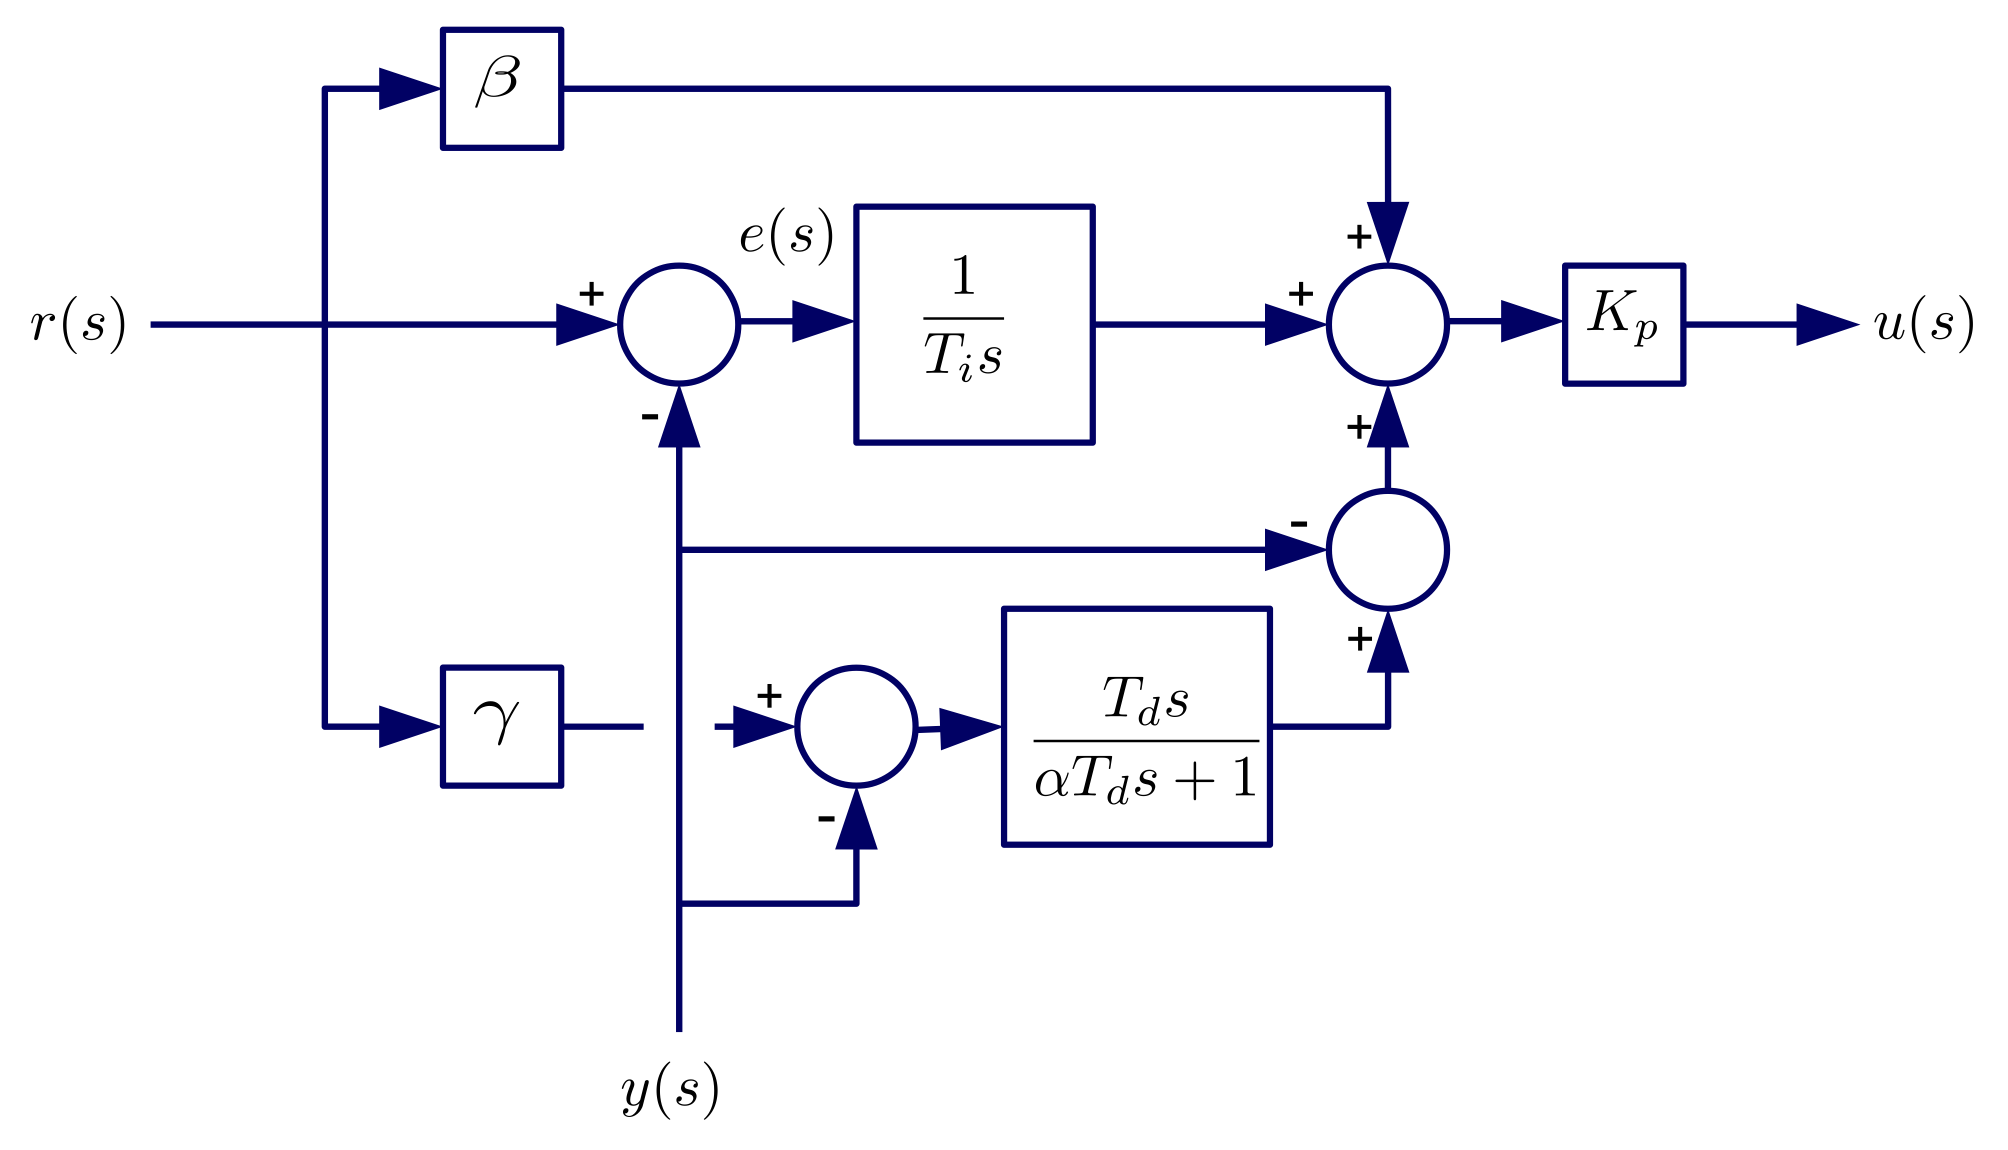
\includegraphics[width=\linewidth]{../figuras/Ch2PID_Schema} 
\caption{Two-degree-of-freedom Standard PID controller.} 
\label{Ch2fig:PID_Schema}
\end{figure}



\begin{itemize}
\item \emph{Standard PID form}: The \emph{textbook} proportional integral derivative control algorithm is the Standard PID whose output is given by the following expression~\cite{astromhagglund1995}:

\begin{equation}
    u(s)= K_p \left( 1 + \frac{1}{T_i s} + \frac{T_d s}{\alpha T_d s+1} \right ) e(s)
    \label{eq:PIDstandard}
\end{equation}

\item \emph{Parallel PID form}: The parallel or \emph{independent gains} PID control algorithm is

\begin{equation}
	u(s) =  \left( K_p + \frac{K_i}{s}+ \frac{K_d s}{\alpha_p K_d s+1}\right) e(s)
\end{equation}

\noindent where each control action has its own independent gain. The gains of the parallel form can be easily related to the gains for the standard form. Whereas the proportional gain is the same, for the integral and derivative gains we have:

\begin{equation}
K_i=\frac{K_p}{T_i} \hspace{2cm}  K_d=K_pT_d 
\end{equation} 

\item \emph{Series PID form}: The  series or \emph{interacting} implementation of the PID algorithm corresponds to the serial connection of a PI and a PD controller. The resulting transfer function is

\begin{equation}
	u(s) = K'_p \left( \frac{T'_i+1}{T'_i s}\right) \left(\frac{T'_d s + 1}{\alpha' T'_d s +1}\right)e(s)
\end{equation}

In this case, parameters are denoted with a prime in order to distinguish them from the standard form ones. As a first difference with the previous formulations, it can be observed that with the series form we can not have complex conjugate zeros. If, for simplicity, we assume the ideal case, $\alpha=\alpha'=0$, a series PID controller equivalent to a Standard one would exists only for $T_i \ge 4 T_d$ (this ensures the Standard PID does not have complex conjugate zeros).

\item \emph{Filtered ideal PID form}: This formulation arises also as an alternative to the mentioned implementation problems with the ideal derivative. In this case, the overall control variable is filtered:

\begin{equation}
	u(s) =  K^*_p \left(1+ \frac{1}{T^*_i s} + T^*_d s  \right) \left(\frac{1}{T_f s+1}\right) e(s)	
\end{equation} 

In this case, parameters are denoted with a star in order to distinguish them from the standard and series form ones. Notice that the controller variable filter introduces the filter time constant $T_f$ as an additional controller parameter. This fact will make the relationship of this controller formulation parameters with the previous ones not so straightforward. It will be presented later on on a more general framework. 
\end{itemize}



\subsection{Reference Processing and 2-DoF PID}
\label{sec:3.2}

The previous PID controller formulations can be improved by introducing some considerations on the processing of the reference signal. The first one is regarding the effect of a step change, $\Delta r$ in the derivative part. Considering, for simplicity, a PD controller, an instantaneous change $\Delta u$ in the control signal will be generated. This instantaneous change will be of magnitude

\begin{equation}
\Delta u = K_p \left ( 1 +\frac{1}{\alpha} \right ) \Delta r \xrightarrow[\alpha=0.1]{}\Delta u = 11 K_p \Delta r
\end{equation} 

This is known as the \emph{derivative kick}. In order to avoid this, it is suggested to feed the derivative with just the output signal.  In this case, the PD controller will take the form

\begin{equation}
u(s)=K_p e(s) - K_p\frac{T_ds}{\alpha T_d s+1} y(s)
\end{equation}

Along the same lines as with the derivative term, a sudden change of magnitude $\Delta r$ in the reference signal generates an instantaneous change $\Delta u$ in the control signal given by $\Delta u = K_p \Delta r$. Therefore, for a relatively high controller gain an excessively abrupt change in the actuator may be demanded. As this is an undesirable feature, the reference signal, in the proportional control action, is recommended to be scaled by a factor $\beta$ known as the \emph{set-point weighting} factor.  The proportional part of the controller is therefore rewritten as

\begin{equation}
u(s)=K_p(\beta r(s) - y(s))
\end{equation}

By choosing $\beta < 1$, the control signal instantaneous change can be scaled down to $\Delta u = K_p \beta \Delta r$  without the need to reduce the controller gain. 

When the \emph{set-point weighting} factor is considered into the PID controller implementation, the resulting controller is said to have two-degrees-of-freedom (2-DoF) as a different processing of the reference and feedback signal is allowed. In such case, the 2-DoF versions of the previously presented PID controller formulations, also considering the avoiding of the derivative kick, results as:

\subsection{2-DoF PID Controller Algorithms Conversion}
As it can be observed from the presented PID formulations, whereas the reference controller aspect $C_r(s)$ takes the same form in all formulations, it is the feedback part $C_y(s)$  that prevents a direct translation of the controller parameters from one formulation to another. This is important because some of the existing tuning rules have been conceived for a specific PID formulation. Due to the possibility that the PID algorithm of the controller to tune be different to the one considered by the tuning rule to use, it is necessary to have conversion relations to obtain ``equivalent'' parameters between two or more of them~\cite{alfaroetfa2012-2} \cite{vilanova2017WEE}. In what follows, we present conversion formulae to get the controller parameters for one specific PID formulation starting from the parameters got for another different one. In order to be as general as possible, the conversion formulae is presented for the more generic 2-DoF PID controller formulations just presented above.


\section{Normalised Representations}
\label{sec:3}

The design approach that is to be presented in the following chapters is applied to controlled processes represented by stable over-damped models. These models encompass from first order to double pole stable models. For control system performance analysis and controller tuning it is convenient to work with dimensionless parameters to made it non dependent on the controlled process time scale and gain. Therefore in this section the process model as well as controller transfer functions to be considered will rewritten in their normalised form in terms of dimensionless parameters.  Therefore, in this book, all the results are based on normalised transfer function models as well as the corresponding normalized controller parameters. In this way we ensure that controller design is consistent from the point of view of being aplicable to all transfer function models equivalent to the normalised one but to a time-scaling.  An additional advantage is that the number of process model transfer function do have one parameter less.\\

\subsection{Process Model Normalisation}
\label{sec:3.2}

The \emph{over-damped} controlled process (first- and second-order) are represented by a linear model given by the transfer function presented in (\ref{Ch2eq:SOPTD})

\begin{equation}
	P(s) = \frac{K \me^{-L s}}{(T s+1)(a T s+1)}, \ \ \theta_p=\left\{K, T, a, L \right\}, 
\end{equation}

\noindent where $K$ is the model gain, $T$ the main time constant, $a$ the ratio of the two time constants ($0 \leq a \leq 1.0$), and $L$ the dead-time.\\

Using the controlled process model gain $K$, and time constant $T$, as well as the transformation $\hat s \doteq T s$, the controlled process \eqref{Ch2eq:SOPTD} can be expressed in normalised form as follows:
\begin{equation}
	\hat P(\hat s) = \frac{\me^{-\tau_L \hat s}}{(\hat s +1)(a \hat s +1)}, \ \ \tau_L \doteq \frac{L}{T}, 
	\label{Ch2eq:SOPTD_n}
\end{equation}

\noindent where $\tau_L$ is the normalised (dimensionless) dead-time.\\

The over-damped second-order plus dead-time (SOPDT) \eqref{Ch2eq:SOPTD_n} model has two normalised parameters, $\hat{\theta}_p = \{a, \tau_L\}$.  For the particular case of the first-order plus dead-time (FOPDT) model ($a=0$) it has only one, $\hat{\theta}_p = \tau_L$. Using the same procedure normalised models are obtained for the other processes.\\


\subsection{Controller Normalisation}
\label{sec:3.3}

Regarding the controller, to consider the control retransfer function alone does not make sense. It has to be considered in conjunction with the process model transfer function to be controlled. Therefore, according to the normalisation of the process model, the controlled transfer function has also to be scaled. This will define the normalised controller parameters. Next we consider the normalization of the \emph{Standard 2DoF PID controller} $PID_2$ from where the normalized parameters of other 2DoF PID control algorithms can be found.

For example, the output equation of the normalized version of the \emph{Standard 2DoF PID controller} $PID_2$ in \eqref{eq:PIDstandard}, with the $\hat s \doteq T s$ transformation, is given by
\begin{equation}
	u(\hat s) = \kappa_p \left\{\beta r(\hat s)-y(\hat s) + \frac{1}{\tau_i \hat s} \left[r(\hat s)-y(\hat s)\right] - \left(\frac{\tau_d \hat s}{\alpha \tau_d \hat s+1}\right) y(\hat s)\right\},
\end{equation}

\noindent with parameters $\hat{\theta}_c = \left\{\kappa_p, \tau_i, \tau_d, \alpha, \beta \right\}$. Therefore,  for \emph{over-damped first-} and \emph{second-order plus dead-time},  models, using the corresponding model parameters the associated $PID_2$ controllers parameters can be expressed in normalised form as follows:

\begin{equation}
	\kappa_p \doteq K K_p, \ \ \tau_i \doteq \frac{T_i}{T}, \ \ \tau_d \doteq \frac{T_d}{T} 
	\label{Ch2eq:PIDNormalized}
\end{equation}

In case the controller is implemented as a \emph{PID Parallel controller} the corresponding normalized parameters are:
\begin{equation}
	\kappa_p \doteq K K_p, \ \ \kappa_i \doteq K K_i T, \ \ \kappa_d \doteq \frac{K K_d}{T}.	
\end{equation}


